\section{Results}\label{sec:results}
\subsection{Redshift Accuracy}
We compare four methods on the same \NTest\ held-out spectroscopic galaxies
(Table~\ref{tab:results}). For each method, we use the posterior median
$z_{50}$ as the point estimate and define the normalized residual
$r=(z_{50}-z_{\rm spec})/(1+z_{\rm spec})$. We report the median bias
$b={\rm median}(r)$, robust scatter
$\sigma_{\rm NMAD}=1.4826\,{\rm median}|r-b|$, and outlier fraction
$\eta=P(|r|>0.15)$.

\begin{deluxetable*}{lrrrrrr}
\tablecaption{Performance on the same 5,083 held-out spectroscopic galaxies.\label{tab:results}}
\tablewidth{0pt}
\tablehead{\colhead{Method} & \colhead{$N_{\rm train}$} & \colhead{$b$} & \colhead{$\sigma_{\rm NMAD}$} & \colhead{$\eta$ (\%)} & \colhead{$C_{68}$ (\%)} & \colhead{$C_{95}$ (\%)}}
\startdata
Bootstrapped flow & 111,952 & -0.0064 & 0.0178 & 2.81 & 68.6 & 94.7 \\
Broadband flow & 22,604 & +0.0001 & 0.0210 & 3.07 & 66.0 & 94.0 \\
EAZY, supplied R prior & \nodata & -0.0017 & 0.0285 & 10.11 & 59.9 & 85.6 \\
LePhare, full COSMOS & \nodata & -0.0028 & 0.0100 & 2.30 & 56.3 & 82.0 \\
\enddata
\tablecomments{All point estimates are posterior medians; $C_\alpha$ is equal-tailed interval coverage. The first three methods use six broadband measurements at inference; released LePhare uses the full deep COSMOS photometry and is the training teacher. EAZY is not calibrated on this population. An ellipsis indicates no training set fitted in this experiment, not absence of prior calibration in the released methods.}
\end{deluxetable*}


The bootstrapped flow achieves $\sigma_{\rm NMAD}=\FlowScatter$, compared
with \SpecScatter\ for the broadband flow: a \ScatterGainSpec\% reduction.
The paired-bootstrap 95\% interval for the scatter difference is
$[-0.0040,-0.0024]$. Its outlier fraction is 2.81\%, compared with 3.07\%
for the broadband flow. This difference is not significant: its 95\%
interval spans $[-0.55,+0.08]$ percentage points. The bootstrapped flow also
has a larger absolute bias ($-0.0064$ versus $+0.0001$) and normalized
root-mean-square residual (0.158 versus 0.151). Its advantage is in robust
scatter, not every accuracy measure. The flows differ in both training
sample size and selection; this comparison does not separate these effects.

\begin{figure*}[!t]
\centering
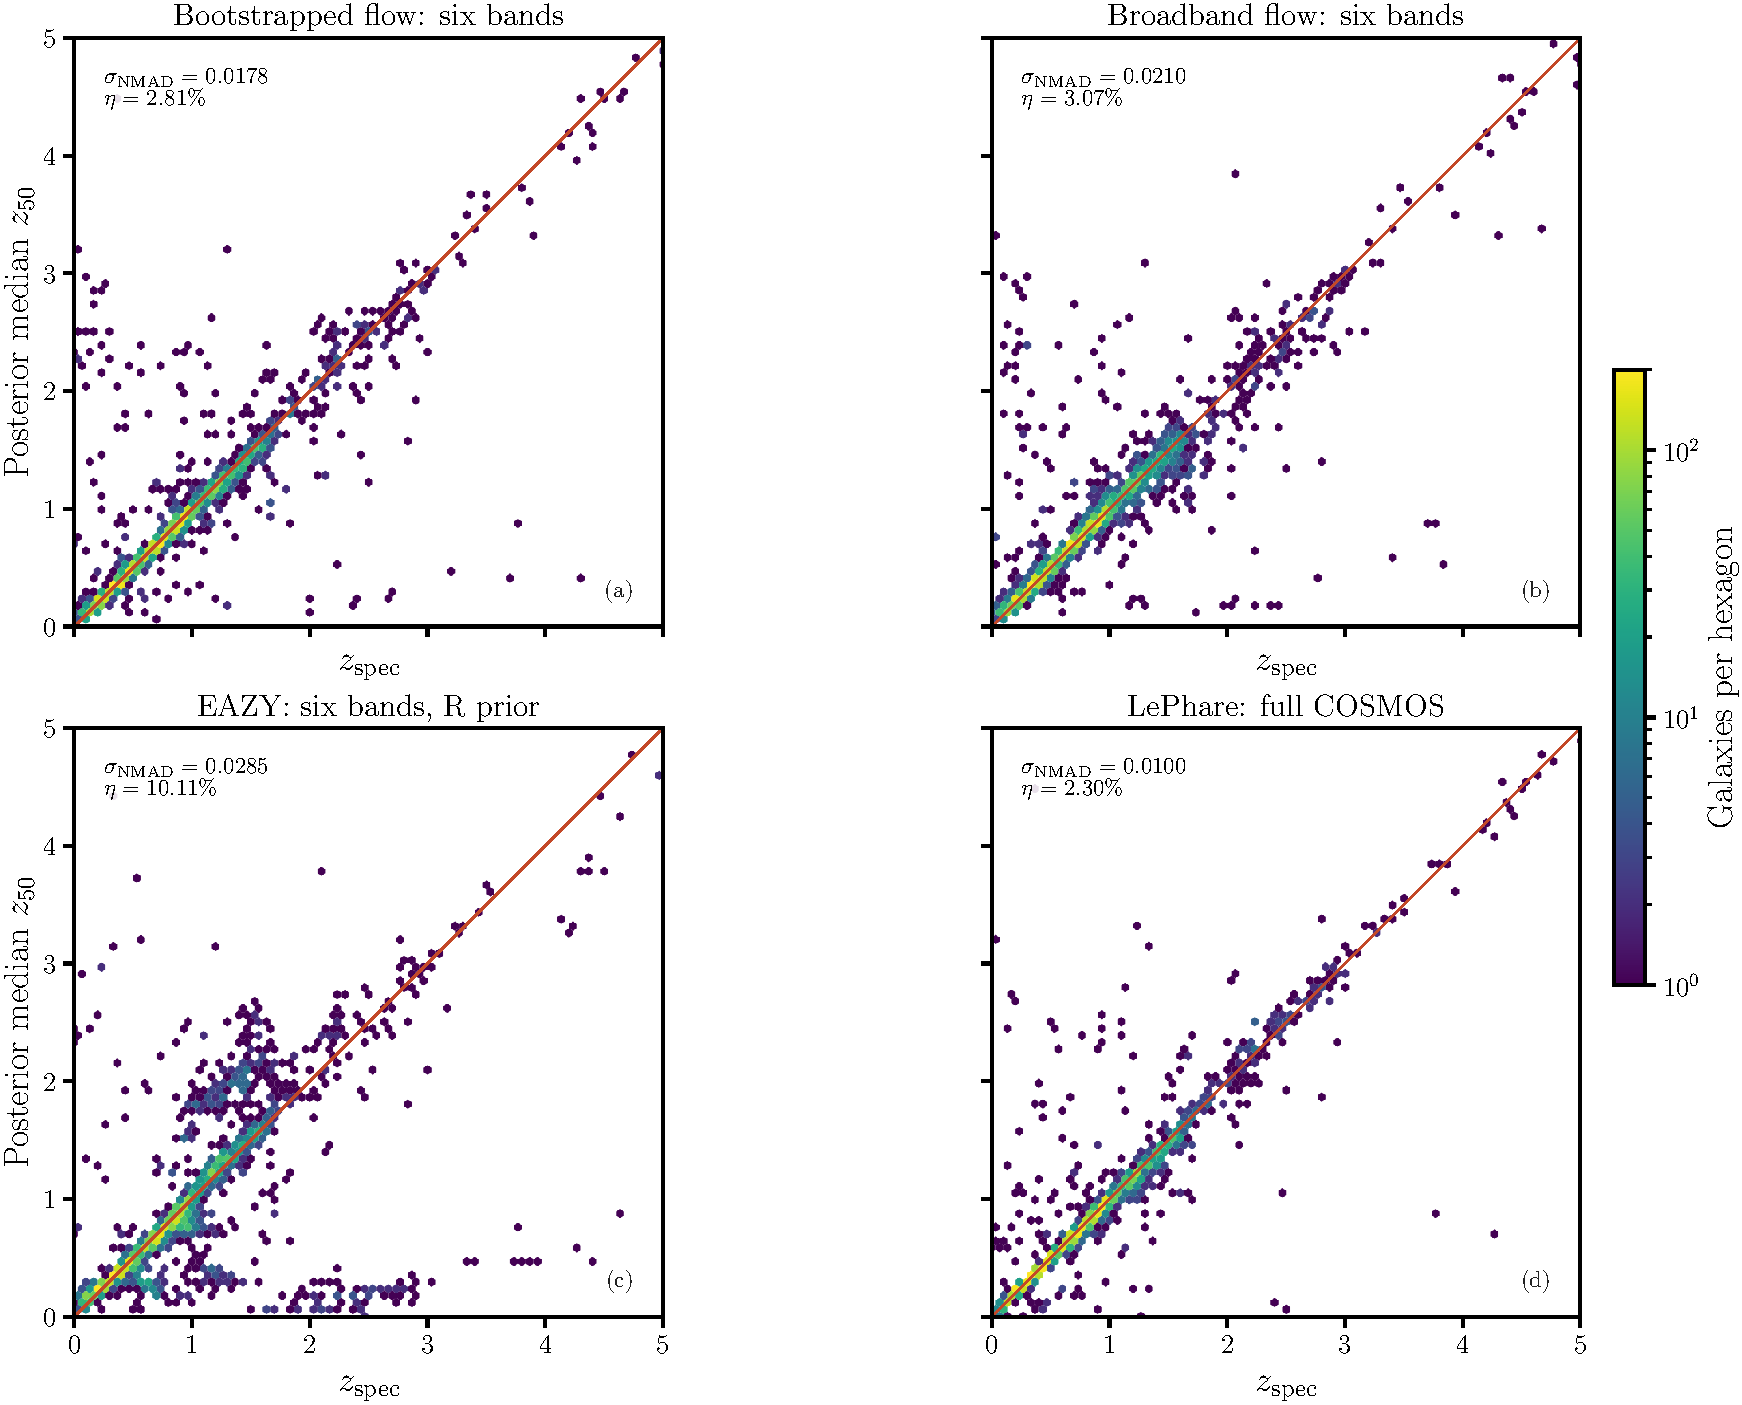
\includegraphics[width=\textwidth,height=0.48\textheight,keepaspectratio]{figures/fig02_accuracy.pdf}
\caption{\label{fig:accuracy}
Posterior-median redshifts for the bootstrapped and broadband flows, EAZY with
its supplied R prior, and full-multiband LePhare, evaluated on the same
\NTest\ galaxies. Colors show counts per hexagon on a shared logarithmic
scale. The diagonal marks equality. Panels show $z<5$; statistics include
the full test sample. LePhare uses the full deep photometry and supplies
the bootstrapped flow's training labels.}
\end{figure*}

Figure~\ref{fig:accuracy} compares the bootstrapped flow with template fitting.
Broadband EAZY gives scatter 0.0285 and 10.11\% outliers. The bootstrapped
flow has \ScatterGainEazy\% lower scatter and \OutlierGainEazy\% fewer
outliers. EAZY is not calibrated on this population, whereas the flow learns
from \NTrain\ probabilistic labels. The comparison therefore applies to
this EAZY configuration, not an optimized template-fitting pipeline.
Using EAZY's posterior mode instead of its median gives scatter 0.0326
and 12.02\% outliers and does not reverse the comparison.

Full-multiband LePhare gives lower scatter (0.0100) and fewer outliers
(2.30\%) than the bootstrapped flow. Its catalog point estimates give
nearly identical results to the PDF medians. This is consistent with the
additional information in the deep multiband measurements, although we
cannot separate information loss from approximation errors in the flow.

\subsection{Uncertainty Calibration}
We measure equal-tailed interval coverage,
\begin{equation}
C_\alpha=\frac{1}{N}\sum_i
\mathbf1\left\{\frac{1-\alpha}{2}\leq
F_i(z_{{\rm spec},i})\leq\frac{1+\alpha}{2}\right\},
\end{equation}
where $F_i$ is the predicted cumulative redshift distribution.
For representative draws from a calibrated model, $C_\alpha=\alpha$.
Our spectroscopic test sample is selected, so coverage here need not
represent the full photometric population.

\begin{figure}[!htbp]
\centering
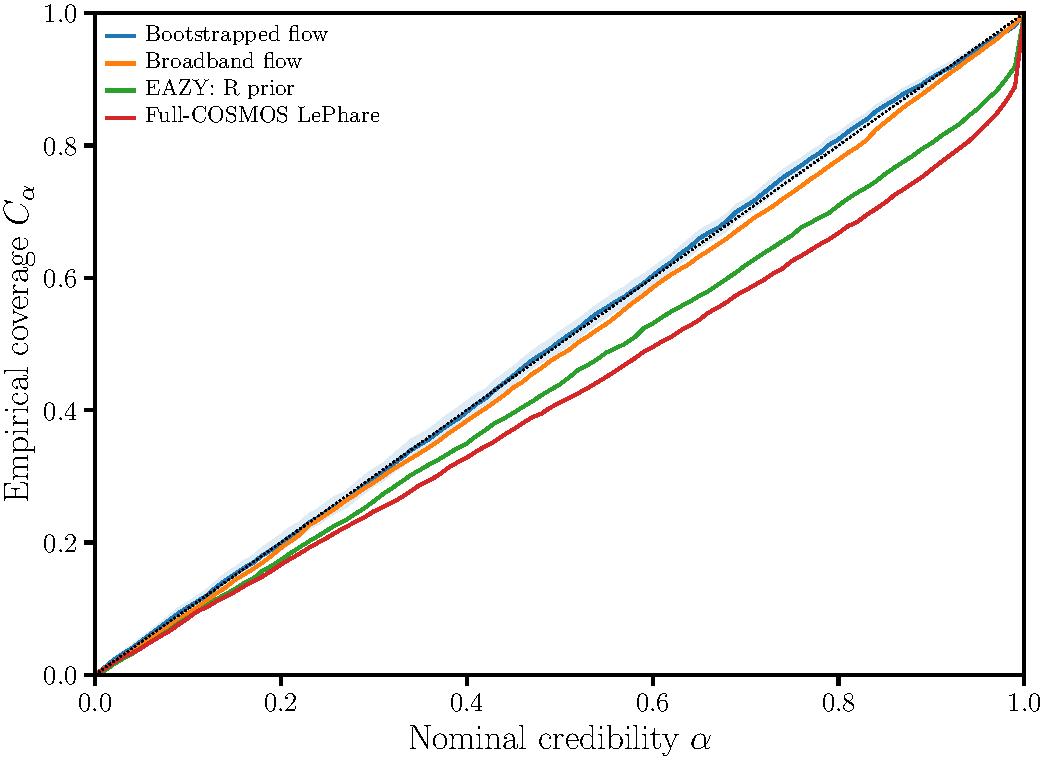
\includegraphics[width=\columnwidth]{figures/fig03_calibration.pdf}
\caption{\label{fig:calibration}
Equal-tailed interval coverage on the common spectroscopic test sample.
The dotted diagonal marks nominal coverage. Shading shows the bootstrapped
flow's 95\% pointwise galaxy-bootstrap interval. Agreement with the diagonal
on this selected sample does not establish population-wide calibration.}
\end{figure}

The bootstrapped flow's nominal 68\% and 95\% intervals contain 68.6\%
and 94.7\% of test redshifts (Figure~\ref{fig:calibration}). The broadband
flow gives 66.0\% and 94.0\%, broadband EAZY gives 59.9\% and 85.6\%,
and full-multiband LePhare gives 56.3\% and 82.0\%.
The median 68\% interval width is 0.0643 for the bootstrapped flow and
0.0259 for LePhare. The bootstrapped flow nevertheless has an asymmetric
probability integral transform, $F_i(z_{{\rm spec},i})$, consistent with
its residual bias. Nearly nominal central coverage can hide unequal tail
errors. Broader intervals after transfer do not demonstrate that the flow
corrects errors in its training PDFs.

We also evaluate LePhare on 34,792 secure spectroscopic matches without
the $i<25$ cut. Its 68\% and 95\% intervals contain 55.7\% and 81.8\%
of redshifts. We apply TARP \citep{lemos2023}, which measures PDF mass
within $|z_{\rm spec}-r_0|$ of a random reference $r_0$. We draw 64 references
per galaxy, either uniformly over $[0,10]$ or within $0.25(1+z_{50})$ of
the median, clipped to the PDF support. The global and local TARP curves
differ, indicating that a single width correction may be insufficient.
The undercoverage agrees qualitatively with \citet{weaver2022}, who report
underestimated faint-galaxy uncertainties. Their sample and interval
definition differ from ours, and spectroscopic selection may contribute
to both results. Undercoverage alone does not establish redshift bias.

We estimate 95\% intervals by resampling galaxies: 200 paired resamples for
the flow comparison and magnitude bins, and 300 for template comparisons
and the coverage band. These intervals exclude training variance, spatial
covariance, and uncertainty from spectroscopic selection. Synthetic
calibrated and narrowed-PDF controls, CDF-inversion checks, and
comparisons of direct and cached EAZY outputs verify the numerical procedure.

\subsection{Magnitude Dependence}
\begin{figure}[!htbp]
\centering
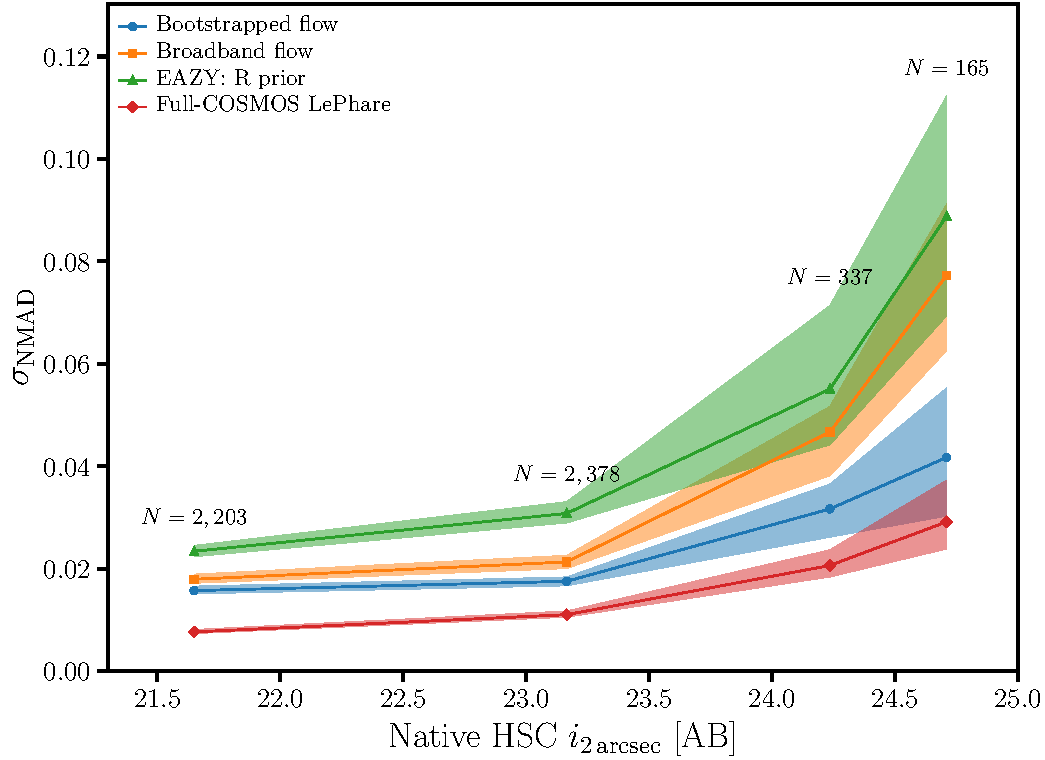
\includegraphics[width=\columnwidth]{figures/fig04_magnitude_dependence.pdf}
\caption{\label{fig:magnitude}
Robust redshift scatter versus native, pre-noise HSC $i$ aperture magnitude.
Points lie at the median magnitude of the test galaxies in each bin, with
identical x-coordinates for all methods. The bins $i<22.5$, $22.5\leq i<24$,
$24\leq i<24.5$, and $24.5\leq i<25$ contain 2,203, 2,378, 337, and 165
galaxies, respectively.
Text labels give the galaxy counts. Shaded bands join the 95\% pointwise
galaxy-bootstrap interval endpoints from 200 resamples.
The faint bins sample the available spectroscopy, not the full photometric
population.}
\end{figure}
Figure~\ref{fig:magnitude} compares scatter in magnitude bins. The
bootstrapped flow has lower scatter than the broadband flow, particularly
in the faint bins. However, only 2.35\% of selected photometric objects at
$24.5\leq i_{\rm ap}<25$ have qualifying spectroscopy, and only 165 enter
the test set. The faint-end comparison therefore remains limited by
spectroscopic selection.

At $z_{\rm spec}>2$, the test sample contains 167 galaxies. The bootstrapped
and broadband flows have nearly identical scatter, 0.0547 and 0.0544,
respectively. Their 68\% coverages are 63.5\% and 70.7\%.
Coverage within true-redshift bins need not be nominal even for a calibrated
posterior. Redshift, magnitude, and spectroscopic selection also covary,
so the aggregate improvement does not establish a high-redshift advantage.
